\documentclass[10pt]{article}

\usepackage
{
	tkz-graph,
	pgfplots,
	hyperref
}

\begin{document}

1. Here some graph just for "illustration / practice" purpose. \hfill \vspace{2.5 mm}

	\begin{tikzpicture}
		\begin{axis} [axis lines = left, xlabel = $x$, ylabel = $f(x)$]
			\addplot[color = blue] {exp(x)};
		\end{axis}
	\end{tikzpicture}	

\vspace{5 mm}

2. A $3D$ example from \href{https://www.overleaf.com/learn/latex/pgfplots_package#Plotting_mathematical_expressions}{Overleaf}:- \hfill \vspace{2.5 mm}

	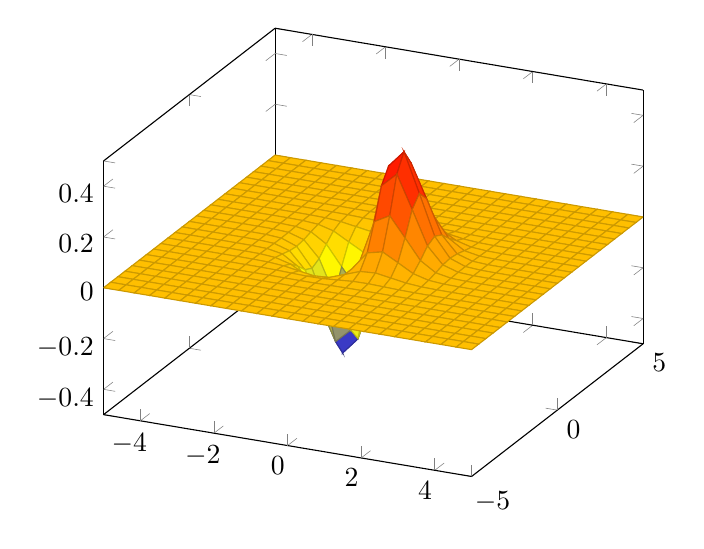
\begin{tikzpicture}
		\begin{axis}
			\addplot3[surf] {exp(-x^2-y^2)*x};
		\end{axis}
	\end{tikzpicture}

\pagebreak

3. Complexity Analysis Graph by BIG-O notation. \hfill \vspace{2.5 mm}

	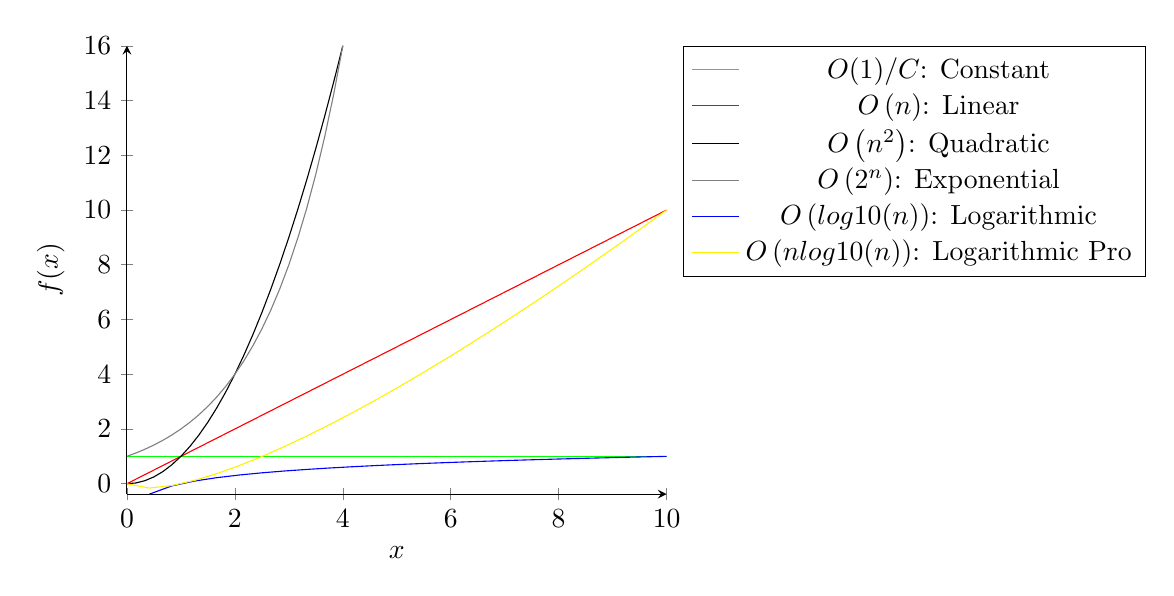
\begin{tikzpicture}
	
		\begin{axis} [
						axis lines = left,
						xlabel = $x$,
						ylabel = $f(x)$,
						legend pos = outer north east,
						xtick = {0, 2,...,10},
						ytick = {0, 2,...,16}
					 ]
			\addplot[green, domain = 0:10] {1};
			\addplot[red, domain = 0:10] {x};
			\addplot[black, domain = 0:4] {x^2};
			\addplot[gray, domain = 0:4] {2^x};
			\addplot[blue, domain = 0:10] {log10(x)};
			\addplot[yellow, domain = 0:10] {x*log10(x)};
			
			\legend{$O(1) / C$: Constant, $O\left(n\right)$: Linear, $O\left(n^2\right)$: Quadratic, $O\left(2^n\right)$: Exponential, $O\left(log10(n)\right)$: Logarithmic, $O\left(nlog10(n)\right)$: Logarithmic Pro}
		\end{axis}
		
	\end{tikzpicture}

4. For $f(x)=ax^2+bx+c$ \hfill \vspace{2.5 mm}
	\begin{tikzpicture}
	
		\begin{axis} [
						axis lines = left,
						xlabel = $x$,
						ylabel = $3x^2+2x+1$,
						legend pos = outer north east,
						xtick = {0, 1,...,4},
						ytick = {0, 5,...,55}
					 ]
			\addplot[red!70!blue!40, domain = 0:4] {3*x^2+2*x+1};
		\end{axis}
		
	\end{tikzpicture}
	
\end{document}